\documentclass{article}
\usepackage[T2A]{fontenc}
\usepackage{amsmath,amsthm} 
\usepackage[utf8]{inputenc}
\usepackage{hyperref}
\usepackage[english,russian]{babel}
\everymath{\displaystyle}
\usepackage[usenames]{color}
\usepackage{graphicx}
\usepackage{enumitem}
\usepackage{epigraph}
\usepackage{xcolor}

\usepackage{geometry}
\geometry{
    a4paper,
    top=20mm, 
    right=1cm,
    bottom=20mm, 
    left=1cm
}

\newcommand{\lin}{Lin}

\usepackage{fancyhdr}
\usepackage{amsfonts}
\pagestyle{fancy}
\fancyhead{}
\fancyfoot[C]{\thepage}

\renewcommand{\headrulewidth}{0pt}
\usepackage{tikz}
\usepackage{tikzsymbols}
\usepackage{textcomp,latexsym,pb-diagram,amsopn}
\usepackage{gnuplottex}

\newtheoremstyle{problemstyle}  % <name>
{3pt}                                               % <space above>
{3pt}                                               % <space below>
{\normalfont}                               % <body font>
{}                                                  % <indent amount}
{\bfseries\itshape}                 % <theorem head font>
{\normalfont\bfseries:}         % <punctuation after theorem head>
{.5em}                                          % <space after theorem head>
{}                                                  % <theorem head spec (can be left empty, meaning `normal')>
\theoremstyle{problemstyle}
\newtheorem{problem}{Задача}[section]

\newcommand\lword[1]{\leavevmode\nobreak\hskip0pt plus\linewidth\penalty50\hskip0pt plus-\linewidth\nobreak\textbf{#1}}
\title{\textbf{Теория вероятностей} \\ Домашнее задание \textnumero 1}
\author{Федоров Егор, P3215, вариант 19}
\date{}

\begin{document}
\maketitle
\section{Рябушко 18.1}
\begin{problem}
    Сколькими способами можно смоделировать флаг,
    состоящий из трех горизонтальных полос различных цветов,
    если имеется материал пяти различных цветов?

    \[ 
        A_5^3 = 5 \cdot 4 \cdot 3 = 60
    \]
\end{problem}

\begin{problem}
    Из коробки, содержащей карточки с буквами <<о>>, <<н>>, <<к>>, <<ь>>,
    наугад вынимают одну карточку за другой и располагают в порядке извлечения.
    Какова вероятность того, что в результате получится слово конь.

    \[
        \frac{1}{4 \cdot 3 \cdot 2 \cdot 1} \approx 0.417
    \]
\end{problem}

\begin{problem}
    Вероятность выигрыша по лотерейному билету первого выпуска равна 0,2, второго – 0,3.
    Имеется по два билета каждого выпуска. Найти вероятность того, что выиграют:
    а) три билета; б) не менее трех билетов; в) менее трех билетов.

    \begin{enumerate}[label=\alph*]
        \item $ P(a) = (2 \cdot 0.2 \cdot 0.2 \cdot 0.3 \cdot 0.7) + (2 \cdot 0.2 \cdot 0.3 \cdot 0.3 \cdot 0.8) = 0.0456 $

        \item $ P(b) = P(a) + 0.2 \cdot 0.2 \cdot 0.3 \cdot 0.3 = 0.0492 $ 

        \item $ P(c) = 1 - P(b) = 0.9508$ 
    \end{enumerate}
\end{problem}

\begin{problem}
    Телеграфное сообщение состоит из сигналов «точка» и «тире»,
    они встречаются в передаваемых сообщениях в отношении 5 : 3.
    Статические свойства помех таковы, что искажаются в среднем
    2/5 сообщений «точка» и 1/3 сообщений «тире».

    Найти вероятность того, что:
    \begin{enumerate}
        \item передаваемый сигнал принят;
        \item принятый сигнал – «тире»
    \end{enumerate}

    \begin{enumerate}
        \item $ \frac{5}{8} \cdot \frac{3}{5} + \frac{3}{8} \cdot \frac{2}{3} = 0.625 $

        \item $ \frac{5}{8} \cdot \frac{2}{5} + \frac{3}{8} \cdot \frac{2}{3} = 0.5 $
    \end{enumerate}
\end{problem}

\begin{problem}
    Вероятность поражения цели при одном выстреле равна 0,4.
    Произведено 8 выстрелов.
    Найти вероятность поражения цели:
    \begin{enumerate}
        \item три раза;
        \item наивероятнейшее число раз;
        \item хотя бы один раз
    \end{enumerate}

    \begin{enumerate}
        \item $C_8^3 \cdot (0.4)^3 \cdot (0.6)^5 \approx 0.2787$
        \item Наивероятнейшее число раз: $\lfloor 0.4 \cdot 8 \rfloor = 3$,
            поэтому ответ совпадает с предыдущим пунктом. $P \approx 0.2787$
        \item Найдем вероятность поражения цели 0 раз:
            $ P' = C_8^0 \cdot (0.4)^0 \cdot (0.6)^8 \approx 0.01679 $.
            Тогда искомая вероятность $P$ равна
            $P = 1 - P' \approx 0.9832 $
    \end{enumerate}
\end{problem}

\begin{problem}
    Вероятность появления события в каждом из 21 независимого испытания равна 0,7.
    Найти вероятность того, что событие наступит не менее 11 раз.

    \[
        P_{21}(11 \leq m \leq 21) =
        \Phi \left( \frac{21 - 21 \cdot 0.7}{\sqrt{21 \cdot 0.7 \cdot 0.3}} \right)
        -
        \Phi \left( \frac{11 - 21 \cdot 0.7}{\sqrt{21 \cdot 0.7 \cdot 0.3}} \right)
        =
        \Phi \left(3\right)
        -
        \Phi \left(1.76\right)
        =
        \Phi (3) + \Phi(1.76)
        =
        0.93435
    \]
\end{problem}

\section{Рябушко 18.2}

\begin{problem}
    Найти закон распределения указанной дискретной СВ $X$
    и ее функцию распределения $F(x)$.
    Вычислить математическое ожидание $M(X)$,
    дисперсию $D(X)$ и среднее квадратичное
    отклонение $\sigma(X)$.
    Построить график распределения $F(x)$.

    Рабочий обслуживает четыре станка.
    Вероятность выхода из строя в течение смены для первого станка равна 0,6,
    для второго – 0,5, для третьего – 0,4, для четвертого – 0,5;
    СВ $ X $ – число станков, вышедших из строя за смену.

    \[ 
        P(0) = 0.4 \cdot 0.5 \cdot 0.6 \cdot 0.5 = 0.06
    \]
    \[ 
        P(1) =
        0.6 \cdot 0.5 \cdot 0.6 \cdot 0.5 +
        0.4 \cdot 0.5 \cdot 0.6 \cdot 0.5 +
        0.4 \cdot 0.5 \cdot 0.4 \cdot 0.5 +
        0.4 \cdot 0.5 \cdot 0.6 \cdot 0.5
        = 0.25
    \]
    \[
        P(3) =
        0.4 \cdot 0.5 \cdot 0.4 \cdot 0.5 +
        0.6 \cdot 0.5 \cdot 0.4 \cdot 0.5 +
        0.6 \cdot 0.5 \cdot 0.6 \cdot 0.5 +
        0.6 \cdot 0.5 \cdot 0.4 \cdot 0.5
        =
        0.25
    \]
    \[
        P(4) = 0.4 \cdot 0.5 \cdot 0.6 \cdot 0.5 = 0.06
    \]
    \[
        P(2) = 1 - (P(0) + P(1) + P(3) + P(4)) = 0.38
    \]

    \begin{table}[ht]
        \centering
        \begin{tabular}{|c|c|c|}
            \hline
            $X$ & $P(X)$ & $F(X)$ \\
            \hline
            0   & 0.06   & 0.06 \\
            \hline
            1   & 0.25   & 0.31 \\
            \hline
            2   & 0.38   & 0.69 \\
            \hline
            3   & 0.25   & 0.94 \\
            \hline
            4   & 0.06   & 1 \\
            \hline
        \end{tabular}
    \end{table}

    \[
        \pmb{MX = 0.25 \cdot 1 + 0.38 \cdot 2 + 0.25 \cdot 3 + 0.06 \cdot 4 = 2}
    \]
    \[
        MX^2 = 0.25 \cdot 1 + 0.38 \cdot 4 + 0.25 \cdot 9 + 0.06 \cdot 16 = 4.98
    \]
    \[
        \pmb{DX = MX^2 - (MX)^2 = 0.98}
    \]
    \[
        \pmb{\sigma = \sqrt{DX} \approx 0.99}
    \]

    \begin{figure}[ht]
        \centering
        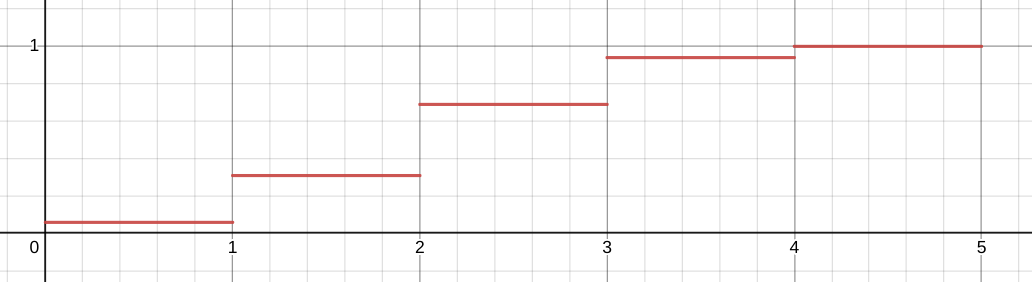
\includegraphics[width=\textwidth]{./18_2_1.png}
        \caption{График $y = F(x)$}
    \end{figure}

\end{problem}
\begin{problem}
    Дана функция распределения $F(x)$ СВ $X$.
    Найти плотность распределения вероятностей $f(x)$, математическое
    ожидание $M(X)$, дисперсию $D(X)$ и вероятность попадания
    СВ Х на отрезок $[a; b]$. Построить графики функций $F(x)$ и $f(x)$.

    \[
        F(x) = \begin{cases}
            0, & x < 1 \\
            \frac{x^2-x}{2}, & 1 \leq x \leq 2 \\
            1, & x > 2
        \end{cases}
        \qquad
        a = 1.5, b = 2
    \]

    \[
        f(x) = \frac{d}{dx} F(x) = \begin{cases}
            0, & x < 1 \\
            x - \frac{1}{2}, & 1 \leq x \leq 2 \\
            1, & x > 2
        \end{cases}
    \]

    \[
        M(X) = \int_{-\infty}^\infty x f(x) \, dx =
        \int_1^2 (x^2 - \frac{1}{2} x) \, dx = \frac{19}{12} \approx 1.58
    \]
    \[
        D(X) = \int_{-\infty}^\infty f(x) (x - M(X))^2 \, dx =
        \int_1^2 \left(x - \frac{1}{2}\right) \left(x - \frac{19}{12}\right)^2 \, dx =
        \frac{11}{144} \approx 0.08
    \]
    \[
        P(1.5 \leq x \leq 2) = F(2) - F(1.5) = 0.625
    \]

    \begin{figure}[ht]
        \centering
        \begin{gnuplot}[terminal=cairolatex, terminaloptions=color, scale=0.6]
            set grid
            set xrange [0:3]
            set xlabel '$x$'
            plot [1:2] x - 1/2 title "$y = f(x)$"
        \end{gnuplot}
        \begin{gnuplot}[terminal=cairolatex, terminaloptions=color, scale=0.6]
            set grid
            set xrange [0:3]
            set xlabel '$x$'
            plot [1:2] x**2 - 1/2*x title "$y = F(x)$"
        \end{gnuplot}
        \caption{График $y = f(x)$ и $y=F(x)$}
    \end{figure}

\end{problem}

\begin{problem}
    При заданном положении точки разрыва снаряда
    цель оказывается накрытой пуассоновским полем осколков с
    плотностью осколков   $\lambda = 2.5$ осколков/$\text{м}^2$. Площадь проекции цели
    на плоскость, на которой наблюдается осколочное поле, равна
    0,8 $\text{м}^2$. Каждый осколок, попавший в цель, поражает ее с полной достоверностью.
    Найти вероятность того, что цель будет поражена.

    Пусть случайная величина $X$ -- количество осколков, попавших
    в цель. Тогда вероятность того, что цель будет поражена --- $P(X \geq 1)$.

    \begin{align*}
        P(X \geq 1) &= 1 - P(X = 0) \\
                    &= 1 - \frac{a^m \cdot e^{-a}}{m!} \\
                    &= 1 - \frac{(2.5 \cdot 0.8)^{0} \cdot e^{- 2.5 \cdot 0.8}}{0!} \\
                    &= 1 - e^{-2} \\
                    &\approx 0.865
    \end{align*}

    \textbf{Ответ:} $0.865$
\end{problem}

\begin{problem}
    Дисперсия каждой из 2500 независимых СВ не превышает 5.
    Оценить вероятность того, что отклонение среднего
    арифметического этих случайных величин от среднего арифметического их
    математических ожиданий не превысит 0,4.

    Пусть событие $Y = \frac{\sum\limits_{i=1}^n x_i}{n} - \frac{\sum\limits_{i=1}^n a_i}{n} \leq \varepsilon$

    \[
        P\left( Y \right) \geq 1 - \frac{D(X)}{n \varepsilon^2}
        = 1 - \frac{5}{2500 \cdot 0.16}
        = 0.9875
    \]

    \textbf{Ответ:} $P \geq 0.9875$
\end{problem}

\section{Чистяков}
\subsection{Глава 2}
\begin{problem}[1]
    Брошено две игральные кости.
    Предполагая, что элементарные события равновероятны,
    найти вероятность событий:
    \[ A = {\text{на 1-й кости выпала 1}}, \bar A \]
    \[ B = {\text{выпала хотя бы одна 6}}, A \bar B \]

    \[
        P(A) = \frac{1}{6}, P(\bar A) = \frac{5}{6}
    \]
    \[
        P(B) = \frac{1}{6} + \frac{1}{6}, P(A \bar B) = P(\text{выпала 1 на первой кости, на второй не выпала 6}) = \frac{1}{6} \cdot \frac {5}{6} = \frac{5}{36}
    \]
\end{problem}

\begin{problem}[2]
    На полке в случайном порядке расставлено $n$ книг, среди которых
    двухтомник Д. Лондона. Предполагая, что различные расположения книг равновероятны,
    найти вероятность того, что оба тома двухтомника расположены рядом.

    \[ P = \frac{(n-2)! 2!}{n!} = \frac{2}{n(n-1)} \]
\end{problem}

\begin{problem}[5]
    Выписана последовательность из $n$ случайных чисел.
    Найти вероятности событий:
    \begin{itemize}
        \item 1-е число -- четное:
            \[ P = \frac{1}{2} \]
        \item Среди $n$ чисел ровно $m$ делятся на 3:
            \[\ P = C_n^m \left(\frac{1}{3}\right)^m \left(\frac{2}{3}\right)^{n-m} \]
        \item Среди $n$ чисел ровно $m+2$ делятся на $3$ и два из них расположены на концах
            последовательности
            \[ P =
                C_{n-2}^m \left(\frac{1}{3}\right)^m \left(\frac{2}{3}\right)^{n-2-m} \cdot \frac{1}{3} \cdot \frac{1}{3} =
                C_{n-2}^m \left(\frac{1}{3}\right)^{m+2} \left(\frac{2}{3}\right)^{n-2-m}
            \]
    \end{itemize}
\end{problem}

\begin{problem}[12]
    Найти вероятность того, что дни рождения 12 человек придутся на разные
    месяцы года.

    \[ P = \frac{12!}{12^{12}} = \frac{479001600}{8916100448256} \approx 5.3723 \cdot 10^{-5} \]
\end{problem}

\begin{problem}[11]
    Из множества чисел $\left\{ -n, -n+1, \ldots, -1, 0, 1, \ldots, n \right\}$
    по схеме случайного выбора с возвращением выбирается 
    два числа $x$ и $y$.
    Пусть $p_n$ -- вероятность того, что $x^2 + y^2 \leq n^2$. Найти $\lim_{n \to \infty} p_n$.

    Рассмотрим систему координат. Так как числа выбираются с возвращением, то
    при $n \to \infty$
    все возможные варианты событий -- квадрат со стороной $2n$ и центром в $(0; 0)$,
    при этом исходы, удовлетворяющие условию $x^2 + y^2 \leq n^2$ --- круг радиуса $n^2$ и центром
    в $(0; 0)$.

    Тогда $\lim_{n \to \infty} P_n = \frac{ \pi n^2 }{4n^2} = \frac{\pi}{4}$
\end{problem}

\subsection{Глава 3}
\begin{problem}[1]
    Брошено две игральных кости. Какова вероятность того, что
    выпало две 3, если известно, что сумма выпавших очков делится на 3?

    Подходящие исходы: $ (1, 2), (1, 5), (2, 1), (2, 4), (3, 3), (3, 6), (4, 2), (4, 5), (5, 1), (5, 4), (6, 3), (6, 6) $.

    Тогда $P = \frac{1}{12}$
\end{problem}

\begin{problem}[3]
    Из множества чисел ${1, 2, \ldots, N}$ по схеме случайного выбора
    без возвращения выбираются три числа. Найти условную вероятность того,
    что третье число попадет в интервал, образованный первыми двумя,
    если известно, что первое число меньше второго.

    Возможно три варианта:
    \begin{itemize}
        \item Третье число меньше первого
        \item Третье число лежит в интервале
        \item Третье число больше второго
    \end{itemize}

    Таким образом, $P = \frac{1}{3}$
\end{problem}


\begin{problem}[4]
    Из урны, содержащей 3 белых и 5 черных шаров, последовательно
    без возвращения извлекают 8 шаров. Пусть $A_0^i$ ($A_1^i$) --- событие,
    состоящее в том, что $i$-й вытянутый шар был черный (белый).
    Найти условные вероятности:
    
    \begin{itemize}
        \item $P(A_1^5 | A_1^1 A_0^2 A_0^3 A_1^4)$.
            Осталось 1 белый шар и 3 черных шара. $P = \frac{1}{4}$
        \item $P(A_0^4 | A_{\alpha_1}^1 A_{\alpha_2}^2 A_{\alpha_3}^3), (\alpha_1, \alpha_2, \alpha_3) = (0, 0, 1), (0, 1, 0), (1, 0, 0)$.
            Так как порядок извлечения не влияет на вероятность извлечения четвертого шара,
            то осталось $2$ белых и $3$ черных шара. Тогда $P = \frac{3}{5}$.
    \end{itemize}
\end{problem}


\begin{problem}[5]
    Доказать, что события $A$ и $\bar B$ независимы,
    если независимы события $A$ и $B$.

    События $B$ и $\bar B$ -- полная группа событий.
    Тогда по формуле полной вероятности:
    \[ P(A) = P(A B) + P (A \bar B) \]
    \[ P(A \bar B) = P(A) - P(A B) = P(A) - P(A) P(B) = P(A) (1 - P(B)) = P(A) P(\bar B) \]
\end{problem}

\begin{problem}[15]
    Предположим, что 5 \% всех мужчин и 0.25 \% всех женщин -- дальтоники.
    Наугад выбранное лицо оказалось дальтоником.
    Какова вероятность, что это мужчина?

    Пусть событие $A$ --- выбранное лицо -- дальтоник, $H_1$ --- выбранное лицо -- мужчина,
    $H_2$ --- выбранное лицо -- женщина.

    Тогда $P(H_1) = 0.5$, $P(A) = P(H_1) \cdot P(A | H_1) + P(H_2) \cdot P(A | H_2) = 0.02625 $

    \[ P(H_1 | A) = \frac{P(A | H_1) \cdot P(H_1)}{P(A)} = \frac{0.5 \cdot 0.05}{0.02625} \approx 0.09523 \]
    
\end{problem}

\subsection{Глава 4}
\begin{problem}[1]
    Два игрока поочередно извлекают шары (без возвращения)
    из урны, содеражщей 2 белых и 4 черных шара.
    Выигрывает тот, кто первым достанет белый шар.
    Найти вероятность выигрыша участника, начавшего игру.

    Участник, начавший игру, выиграет в следующих комбинациях: Б, ЧЧБ, ЧЧЧЧБ.

    \[ P_1 = \frac{2}{6} = \frac{1}{3} \]
    \[ P_2 = \frac{4}{6} \frac{3}{5} \frac{2}{4} = 0.2 \]
    \[ P_3 = \frac{4}{6} \frac{3}{5} \frac{2}{4} \frac{1}{3} \frac{2}{2} = \frac{1}{15} \]
    \[ P = P_1 + P_2 + P_3 = 0.6 \]
\end{problem}

\begin{problem}[4]
    Проведено 10 независимых испытаний, каждое из которых
    заключается в одновременном подбрасывании
    трех игральных костей.
    Найти вероятность того, что в четырех испытаниях появятся в точности
    по две <<6>>.
    \[ P'= C_3^2 \left(\frac{1}{6}\right)^2 \frac{5}{6} = \frac{15}{216} \]
    \[ P = C_4^{10} \left(\frac{15}{216}\right)^4 \left(\frac{201}{216}\right)^6 \approx 0.00317 \]
    
\end{problem}


\begin{problem}[5]
    При передаче сообщения вероятность искажения одного знака
    равна 1/100. В предположении независимости искажения
    знаков найти вероятность того, что сообщение из 5 знаков:

    \begin{itemize}
        \item Не будет искажено:
            \[ P' = \left(\frac{99}{100}\right)^5 \approx 0.9509 \]
        \item Содержит ровно одно искажение:
            \[ P'' = C_5^1 \left(\frac{1}{100}\right)^1 \left(\frac{99}{100}\right)^4 \approx 0.048  \]
        \item Содержит хотя бы два искажения:
            \[ P = 1 - (P' + P'') \approx 0.001 \]
    \end{itemize}
\end{problem}

\begin{problem}[9]
    Найти вероятность того, что в $n$ испытаниях
    схемы Бернулли с вероятностью успеха $p$ появится $m+l$ успехов,
    причем $l$ успехов появятся в последних $l$ испытаниях.

    \[
        P =
        P(\text{m в первых n - l}) \cdot P(\text{l в последних l}) = 
        C_{n-l}^m p^{m}   (1-p)^{n - l - m} \cdot p^l =
        C_{n-l}^m p^{m+l} (1-p)^{n - l -m}
    \]
\end{problem}

\begin{problem}[12]
    На отрезок $[0; 10]$ на удачу брошено 5 точек.
    Найти вероятность того, что две точки попадут в $[0; 2]$, одна
    -- в $[2; 3]$, две -- в $[3; 10]$.

    \[ P =
        \underbrace{\left[ C_5^2 \left(\frac{2}{10}\right)^2 \right]}_{\text{первые две попадут в } [0; 2]} \cdot
        \underbrace{\left[ C_3^1 \frac{1}{10} \right]}_{\text{третья попадет в } [2; 3]} \cdot
        \underbrace{\left[ \left(\frac{7}{10}\right)^2 \right]}_{\text{последние две в } [3; 10]}
        \approx 0.0588
    \]
\end{problem}

\subsection{Глава 5}

\begin{problem}[1]
    Плотность распределения $\zeta$ задана формулами
    \[
        p_\zeta(x) = \begin{cases}
            \frac{C}{x^4}, & x \geq 1 \\
            0, & x < 1
        \end{cases}
    \]

    Найти постоянную $C$, плотность распределения величины $\eta = \ln \zeta$,
    $P (0.5 < \eta < 0.75)$

    \[
        1 =
        \int\limits_{-\infty}^{+\infty} p(x) \, dx =
        C \int\limits_{1}^{+\infty} \frac{1}{x^4} \, dx =
        \frac{C}{3}
    \]
    Значит $\frac{C}{3} = 1 \Rightarrow C = 3$.

    \[
        \ln \zeta < x \Leftrightarrow \zeta < e^x
    \]

    \[
        F_\eta(x) = P(\eta < x) = P(\ln \zeta < x) = P(\zeta < e^x) =
        \int\limits_{1}^{e^x} \frac{3}{t^4} \, dt
    \]

    \[
        p_\eta(x) = F'_\eta(x) = \frac{3}{e^{3x}}, \quad x \geq 0
    \]
    \
    \[
        P(0.5 < \eta < 0.75) =
        \int\limits_{0.5}^{0.75} p_\eta(x) \, dx
        \int\limits_{0.5}^{0.75} \frac{3}{e^{3x}} \, dx \approx
        0.1177
    \]
\end{problem}

\begin{problem}[8]
    Случайные величины $\zeta_1$ и $\zeta_2$ независимы,
    одинаково распределены и имеют показательное распределение:
    $p_{\zeta_1}(x) = p_{\zeta_2}(x) = \alpha e^{- \alpha x}$, $x > 0$.
    Найти плотность распределения их суммы.
    \begin{align*}    
        p_{\zeta_1 + \zeta_2}(x) &= \int\limits_{-\infty}^{+\infty} p_{\zeta_1}(t) p_{\zeta_2}(x - t) \, dt \\
                                 &= \int\limits_{0}^{z} \alpha e^{- \alpha t} \alpha e^{- \alpha (x-t)} \, dt \\
                                 &= \int\limits_{0}^{z} \alpha^2 e^{-ax} \, dt \\
                                 &= \alpha^2 x e^{-ax}
    \end{align*}
\end{problem}



\begin{problem}[13]
    Найти закон распределения суммы двух независимых случайных величин
    $\zeta_1, \zeta_2$, каждая из которых имеет распределение
    Пуассона с параметром $\lambda_1$ и $\lambda_2$ соответственно.

    \[
        p(\zeta_1 = k) = \frac{\lambda_1^k}{k!} e^{-\lambda_1}
        \qquad
        p(\zeta_2 = k) = \frac{\lambda_2^k}{k!} e^{-\lambda_2}
    \]
        \begin{align*}
            p(\zeta_1 + \zeta_2 = k) 
            &= \sum_{i=0}^k p(\zeta_1 = i) \cdot p(\zeta_2 = k - i) \\
            &= \sum_{i=0}^k \frac{\lambda_1^i}{i!} e^{-\lambda_1} \cdot \frac{\lambda_2^{k-i}}{(k-i)!} e^{-\lambda_2} \\
            &= \frac{e^{-(\lambda_1 + \lambda_2)}}{k!} \sum_{i=0}^k C_k^i \lambda_1^i \lambda_2^{k-i} \\
            &= \frac{(\lambda_1 + \lambda_2)^k}{k!} e^{-(\lambda_1 + \lambda_2)}
        \end{align*}

        Значит $\zeta_1 + \zeta_2$ имеет распределение Пуассона с параметром $\lambda_1 + \lambda_2$.
\end{problem}

\begin{problem}[14]
    Обозначим $\tau$ число испытаний в схеме Бернулли до появления
    первого успеха включительно. Найти закон распределения $\tau$.

    Должно произойти $k-1$ провал и $1$ успех,
    причем порядок важен и единственен.
    Значит вероятность того, что $\tau = k:$
    \[ p(\tau = k) = (1-p)^{k-1} \cdot p \]
\end{problem}


\begin{problem}[16]
    Найти закон распределения величины $\tau^{(m)}$, равной числу
    испытаний в схеме Бернулли до появления $m$-го успеха.

    Пусть было проведено $k$ испытаний.
    Значит из них $m$ из них -- успех, $k -m $ -- провал,
    причем порядок $m-1$ успеха и $k-m$ провалов не важен, а
    порядок последнего успеха важен.

    \[
        P(\tau^{(m)} = k) =
        C_{k-1}^{m-1} p^{m-1} (1-p)^{k-m} p = 
        C_{k-1}^{m-1} p^m (1-p)^{k-m}
    \]
\end{problem}
\subsection{Глава 6}

\begin{problem}[1]
    Найти математическое ожидание величины $\tau$, определенной в задаче
    14 гл. 5.

    \[ p(\tau = k) = (1-p)^{k-1} \cdot p \]
    \[
        M \tau =
        \sum_{k=0}^\infty k \cdot p(k) =
        \sum_{k=0}^\infty k p (1-p)^{k-1} =
        p \sum_{k=0}^\infty k (1-p)^{k-1} =
        p \cdot \frac{1}{(q-1)^2} =
        \frac{p}{p^2} =
        \frac{1}{p}
    \]
\end{problem}

\begin{problem}[4]
    Найти $M \tau^{(m)}$ величины $\tau^{(m)}$, определенной в задаче 16 гл. 5.

    \[ p(\tau^{(m)} = k) = C_{k-1}^{m-1} p^m (1-p)^{k-m} \]
    \begin{align*}
        M \tau^{(m)} &= 
        \sum_{k=m}^\infty k p(k) = \\
                     &= \sum_{k=m}^\infty k C_{k-1}^{m-1} p^m (1-p)^{k-m} \\
                     &= p^m \sum_{k=m}^\infty k \frac{(k-1)!}{(m-1)!(k-m)!} (1-p)^{k-m} =  \\
                     &= p^m m \sum_{k=m}^\infty \frac{k!}{m! (k-m)!} \cdot (1-p)^{k-m}  =  \\
                     &= p^m m \sum_{k=m}^\infty C_k^m 1^k (1-p)^{k-m} = \\
                     &= p^m m p^{-m-1} = \frac{m}{p}
    \end{align*}
\end{problem}

\begin{problem}[16]
    По $n$ конвертам случайно разложили $n$ писем различным адресатам.
    Найти вероятность того, что хотя бы одно письмо попадет своему адресату.
    Найти предел этой вероятности при $n \to \infty$.

    Найдем вероятность $P'$ того, что ни одно число не попадет своему адресату.
    Всего есть $n!$ способов сопоставить письмо и конверт.
    Рассмотрим перестановку $\sigma$, при которой ни одно письмо не 
    попало в соответсвующий конверт. Из этого следует, что
    у данной перестановки нет неподвижных точек,
    значит всего таких перестановок $D(n)$ (субфакториал $n$).

    \[
        P'_n =
        \frac{D(n)}{n!} =
        \frac{n! \sum_{k=0}^n \frac{(-1)^k}{k!}}{n!} =
        \sum_{k=0}^n \frac{(-1)^k}{k!}
    \]

    Тогда вероятность того, что хотя бы одно письмо попадет в нужный конверт:
    \[
        P_n =
        1 - P'_n =
        1 - \sum_{k=0}^n \frac{(-1)^k}{k!}
    \]

    \[
        \lim_{n \to \infty} P_n =
        1 - \lim_{n \to \infty} P'_n =
        1 - \lim_{n \to \infty} \sum_{k=0}^n \frac{(-1)^k}{k!} =
        1 - \frac{1}{e} =
        \frac{e-1}{e}
    \]
\end{problem}

\begin{problem}[17]
    В задаче 16 найти математическое ожидание и дисперсию числа $\zeta$
    писем, попавших своему адресату.

    Всего $n$ писем. Вероятность того, что адресант получит письмо --- $\frac{1}{n}$.
    Случайная величина $\zeta = \sum_{k=0}^n A_k$, где $A_k = 1$  если $k$-й адресант
    получил свое письмо, $A_k = 0$ -- иначе.

    \[
        M \zeta =
        M \left(\sum_{k=0}^n A_k\right) =
        \sum_{k=0}^n M (A_k) =
        \sum_{k=0}^n \left( 1 \cdot \frac{1}{n} + 0 \cdot \frac{n-1}{n} \right) =
        1
    \]

    Вычислим $M (\zeta^2)$.

    \[
        M ( \zeta^2) =
        M\left( \sum_{k=0}^n A_k \right)^2 =
        M\left( \sum_{k=0}^n A^2_k + \sum_{i = 0}^n \sum_{j=0}^n A_i A_j \right) =
        M \left( \sum_{k=0}^n A^2_k  \right) + M \left( \sum_{i = 0}^n \sum_{j=i}^n 2 A_i A_j \right) =
    \] 
    \[
        = \sum_{k=0}^n M (A^2_k)  + \sum_{i = 0}^n \sum_{j=i}^n 2 M(A_i A_j) =
        1 + 1 =
        2
    \]

    Тогда $D \zeta = M \zeta^2 - (M \zeta)^2$ = 1

    Ответ: $M \zeta = D \zeta = 1$.
\end{problem}

\begin{problem}[18]
    В $N$ ящиков случайно и независимо друг от друга бросают шары, пока
    не останется пустых ящиков. Обозначим $\nu$ число брошенных шаров.
    Найти $M \nu$.

    Найдем $p(\nu = k)$, $k \geq n$.
    Так как серия бросков обязательно кончается попаданием, нужно
    учесть это в вероятности.
    \[
        p(\nu = k) =
            C_{k-1}^{n-1}
            \left(\frac{1}{n}\right)^n
            \left(\frac{n-1}{n}\right)^{k-n}
    \]

    \begin{align*}
        M \nu &= \sum_{k=n}^\infty k p(k) = \\
              &= \sum_{k=n}^\infty k C_{k-1}^{n-1} \left(\frac{1}{n}\right)^n \left(\frac{n-1}{n}\right)^{k-n} \\
              &= \left(\frac{1}{n}\right)^n \sum_{k=n}^\infty k \frac{(k-1)!}{(n-1)! (k - n)!} \left(\frac{n-1}{n}\right)^{k-n} \\
              &= \left(\frac{1}{n}\right)^n \cdot n \cdot \sum_{k=n}^\infty \frac{k!}{n! (k-n)!} \left(\frac{n-1}{n}\right)^{k-n} \\
              &= \left(\frac{1}{n}\right)^n \cdot n \cdot \sum_{k=n}^\infty C_k^n \left(\frac{n-1}{n}\right)^{k-n} \\
              &= \left(\frac{1}{n}\right)^n n \left(\frac{1}{n}\right)^{-n-1} \\
              &= n^2
    \end{align*}

\end{problem}

\end{document}
